%Goals
%You can choose the most suitable way to take parameters in functions
%You know how to write a lambda with a capture
%You know 5 different ways to react to errors in functions 
%You know how to throw, catch and test exceptions

\section{Functions}
\begin{itemize}
  \itemsep -0.5em 
  \item Functions are always written in lower Camel Case
  \item A function must be declared always in a header file before the function is used
  \item A good function has a maximum of five parameters and does exactly one thing
  \item The call of the function parameters is not defined.
  \item The main function does implicit return a "0".
  \item Auto should not be used as a return type, exceptions are: inline, template or constexpr functions in header files.
  \item Void should not be used as a function parameter
  \item NEVER return a ref to a local variable since it produces a dangling Reference, because the value lives in the stack frame.
\end{itemize}

\subsection{Default Arguments}
A function declaration can provide default arguments for its parameters \textit{from the right.}
\begin{lstlisting}[language=C++]
void incr(int & var, unsigned delta = 1);
// Default arguments can be omitted  calling
int counter {0};
incr(counter); // uses default for delta
\end{lstlisting}

\subsection{Function Overloading}
The same function name can be used for different functions if parameter number or types differ. Function can not be overloaded just by their return type! If only the parameter type is different there might be ambiguities. The resolution fo overloads happens at compile-time = Ad hoc polymorphism.
\begin{lstlisting}[language=C++]
void incr(int & var);
int incr(int & var); // doesn't compile because of same signature
void incr(int & var, unsigned delta);
\end{lstlisting}

\subsection{Reference / Value Arguments}
\textbf{Parameter Declarations}
\begin{center}
	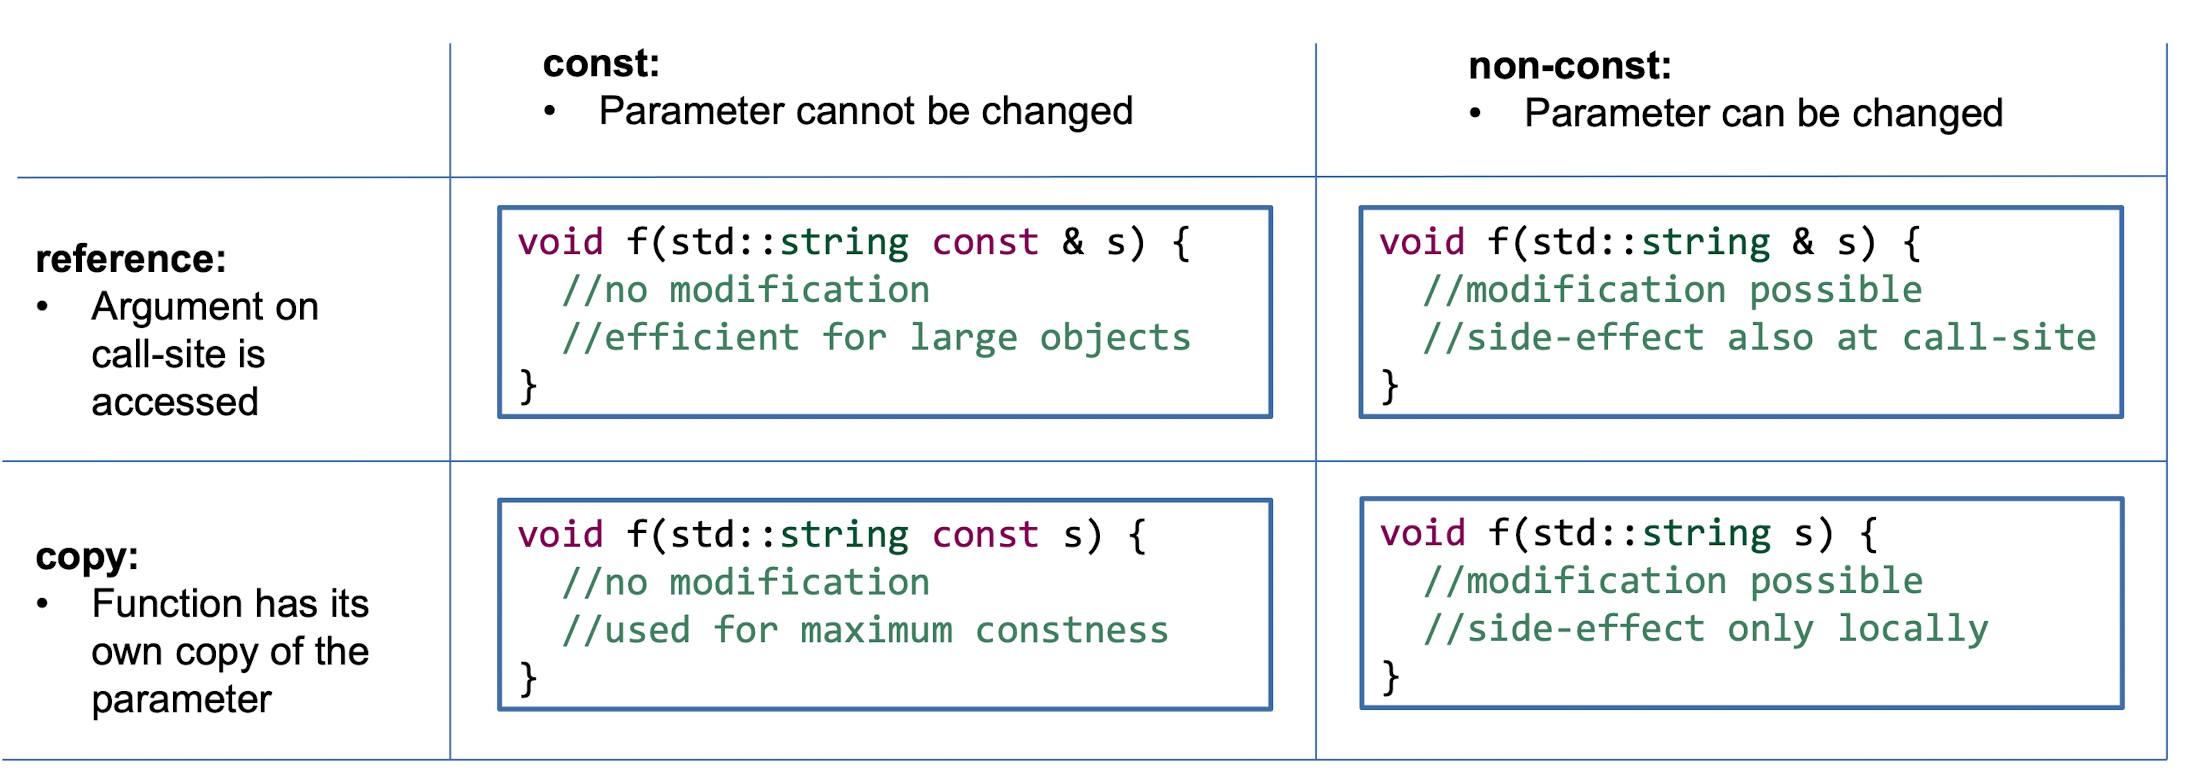
\includegraphics[width=0.75\linewidth]{images/functionparameters}	
\end{center}

\begin{itemize}
  \itemsep -0.5em 
  \item Value Parameter - Default void f(type par);
  \item Reference Parameter - side-effect void f(type \& par);
  \item Const-Reference Parameter - optimisation void f(type const \& par);
  \item Const Value Parameter - Prevent changing the para void f(type const par);
\end{itemize}

\textbf{Function Return Type} \\
\begin{itemize}
  \itemsep -0.5em 
  \item By (Const) Value - default type f(); or type const f();
  \item By Reference - Only return a reference parameter (or a call member variable from a member function) type \& f(); or type const \& f();
\end{itemize}

\textbf{Functions as Parameters} \\
Functions are "first class" objects in C++. You can pass them as augment and you can keep them in reference variables.

\subsection{Variadic Arguments}
Variadic functions take a variable number of arguments. This example is even a template function with variadic arguments.
\begin{lstlisting}[language=C++]
template<typename First, typename...Types> 
void printAll(First const & first, Types const &...rest) {
	std::cout << first;
	if (sizeof...(Types)) {
		std::cout << ", "; 
	} 
	printAll(rest...);
}
\end{lstlisting}


\subsection{Lambdas}
\begin{itemize}
  \itemsep -0.5em 
  \item Can be written into variables \lstinline[language=C++]|auto l = [](); l();|
  \item The smallest lambda is \lstinline[language=C++]|[](){}| the first two brackets are the function object and the round brackets the call.
\end{itemize}

Defining Inline functions. Auto const for function variable for Lambda. [] introduces a Lambda function. Can contain captures: [=] or [\&] to access variables from scope.
\begin{lstlisting}[language=C++]
auto const g = [](char c) -> {
	return std::toupper(c)M
};
g('a');
\end{lstlisting}

\subsubsection{Captures}
Captured variables are imutable default. To change them they have to be declared as \lstinline|mutable|.
\begin{itemize}
	\itemsep -0.5em
	\item \lstinline|[=]| - default implicit capture variables used in body by value
	\item \lstinline|[&]| - default capture variable used in body by reference
	\item \lstinline|[var = value]| - introduce new capture variable with value
	\item \lstinline|[=,& out]| - capture all by copy, out by reference 
	\item \lstinline|[&, = x]| - capture all by reference, but x by copy/value
\end{itemize}
\begin{lstlisting}[language=C++]
// Capturing by value
int x = 5;
auto l = [x]() mutable {
	std::cout << ++x;
};
// Capuring by reference
auto const l = [&x]() {
	std::cout << ++x;
};
\end{lstlisting}

\subsection{Functor}
Functors are types which provide an operation. Functors have an overloaded call operator. Lambdas internally work with functors. The \lstinline|operator()| function can theoretically be overload as often as needed.
\begin{lstlisting}[language=C++]
struct Accumulator {
  int count{0};
  int accumulated_value{0};
  void operator()(int value) {
    count++;
    accumulated_value += value;
  }
	int average() const {
		return accumulated_value / count;
	}
  int sum() const;
};

int average(std::vector<int> values) {
  Accumulator acc{};
  for(auto v : values) { acc(v); }
  return acc.average();
}
int main(int argc, char **argv) {
	std::vector<int> values { 1, 2, 6, 4, 5, 3 };
	std::cout << average(values);
}
\end{lstlisting}


\pagebreak
\section{Exceptions}
An exception can throw any copyable type. No means to specify what could be thrown. No check if you catch an exception that might be thrown at call-site. No meta-information is available as part of the exception. Exception thrown while exception is propagated results in a program abort (not while caught). 

\subsection{Failing Functions}
What should we do, if a function cannot fulfil its purpose?
\begin{enumerate}
  \itemsep -0.5em 
  \item Ignore the error and provide potentially undefined behaviour
  \item Return a standard result to cover the error
  \item Return an error code or error value
  \item Provide an error status as a side-effect
  \item Throw an Exception
\end{enumerate}

\begin{minipage}{0,5\linewidth}
	\textbf{Ignore the Error}
		\begin{itemize}
  			\itemsep -0.5em 
  			\item Relies on the caller to satisfy all preconditions.
  			\item Viable only if not dependent on other resources.
  				\item Most efficient implementation.
  		\item Simple for the implementer but hard for the caller.
		\end{itemize}
	\textbf{Cover the Error with a Standard Result}
		\begin{itemize}
  			\itemsep -0.5em 
  			\item Reliefs the caller from the need to care if it can continue with the default value
  			\item Can hide underlying problems.
  			\item Often better if caller can specify its own default value.
		\end{itemize}
\end{minipage}
\begin{minipage}{0,5\linewidth}
  	\textbf{Error Value} 
  		\begin{itemize}
 			\itemsep -0.5em 
  			\item Only feasible if result domains is smaller than return type
  			\item POSIX defines -1 to mark failure of system calls
  			\item Burden on the caller to check the result
		\end{itemize}
	\textbf{Cover the Error with a Standard Result}  
		\begin{itemize}
  			\itemsep -0.5em
  			\item Requires reference parameter
  			\item (Bad!) Alternative: global variable (POSIX: errno)
  			\item E.g: std::istreams’s states (good(), fail()) is chan- ged as a side-effect of input
		\end{itemize}
\end{minipage}

\subsection{Catching Exceptions}
Principle: Throw by value, catch by const reference. This avoids unnecessary copying and allows dynamic polymorphism for class types.
\begin{lstlisting}[language=C++]
#include <stdexcept> // contains some sublcasses
try {
throw std::logic_error("message");
} catch (type const & e) {
	//Handle type exception 
} catch (type2 const & e) {
	//Handle type2 exception 
} catch (...) {
	//Handle other exception types 
}
\end{lstlisting}
The Standard Library has some pre-defined exception types that you can also use in <stdexcept>. All have a constructor parameter for the "reason" of type std::string. It provides the what() member function to obtain the "reason"
\begin{center}
	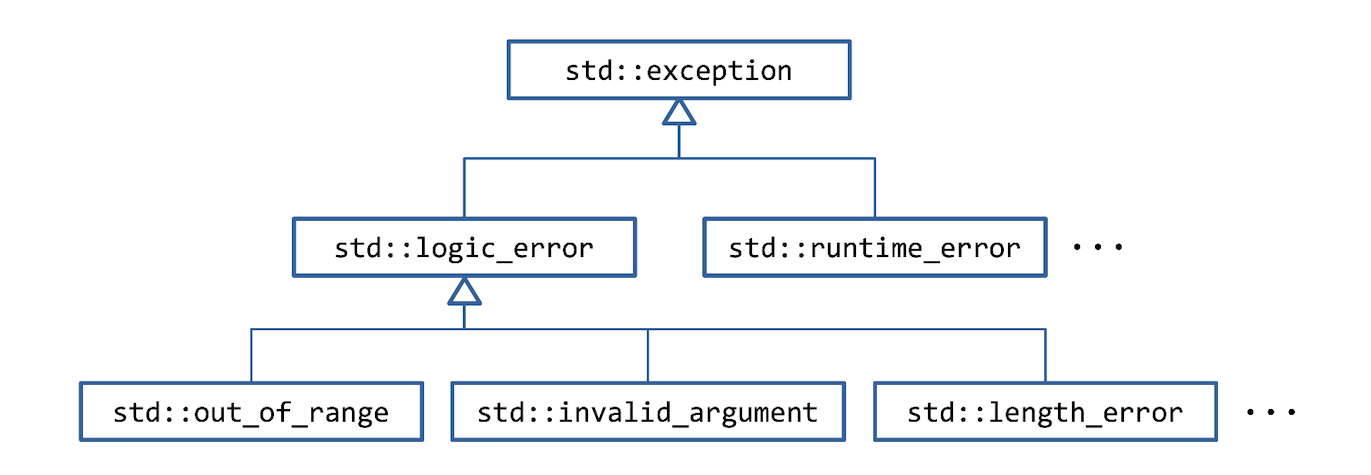
\includegraphics[width=0.75\linewidth]{images/exceptions}
\end{center}

\subsection{Keyword noexcept}
Functions can be declared to explicitly not throw an exception with the noexcept keyword. The compiler does not need to check it.  If an exception is thrown (directly or indirectly) from a noexcept function the program will terminate.

\break